% ============================================================================
% Seções 4 (Resultados) e 5 (Considerações finais) -- continuação de tp3-heu.pdf
% Pacotes necessários no preâmbulo: graphicx, booktabs.
% Figura: figuras/artigo_painel.pdf (gerada por Execucao Oficial/analise/figuras_artigo.py).
% Tabelas geradas por Execucao Oficial/analise/tabelas_latex.py (números sem redigitação).
% ============================================================================

\section{Resultados}

As 25.620 execuções previstas foram concluídas sem falhas, e a reavaliação independente das rotas (vértices, clusters, orçamento e prêmio) não encontrou divergências. Com limite de 600~s, a formulação exata provou 234 dos 294 ótimos de T1 a T3 e melhorou o BKS de 11 instâncias (Tabela~\ref{tab:exato}); nenhuma heurística superou um ótimo provado. A compilação não usou \texttt{-O2}, e as 86 últimas instâncias da exata rodaram com 4 processos simultâneos, e não 5, por falta de memória.

\begin{figure}[t]
\centering
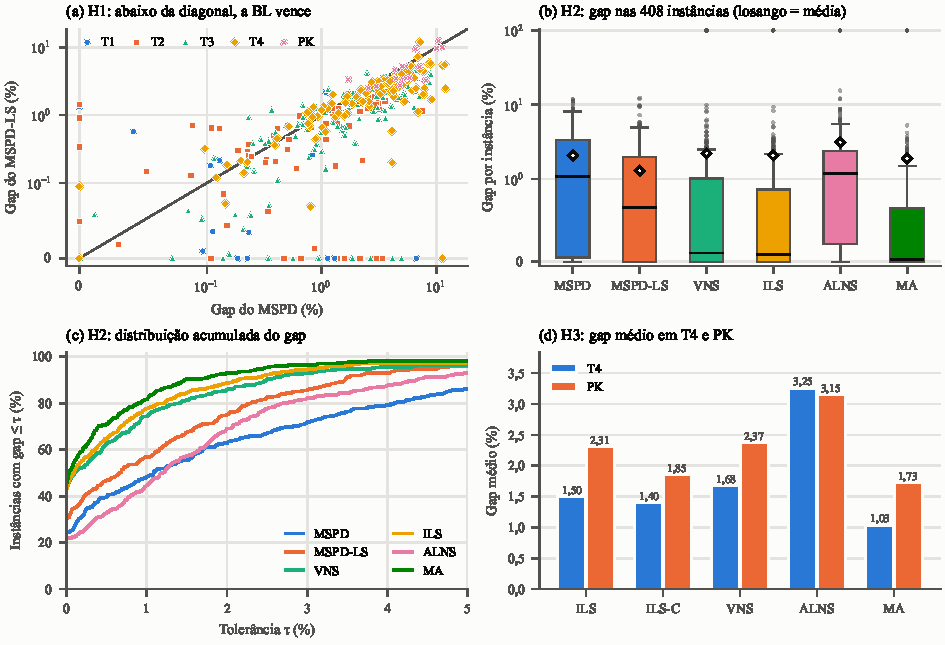
\includegraphics[width=0.92\textwidth]{figuras/artigo_painel.pdf}
\caption{(a) H1: gap médio por instância do MSPD ($x$) e do MSPD-LS ($y$), em escala log-linear; (b) e (c) H2: boxplot e distribuição acumulada do gap médio por instância; (d) H3: gap médio em T4 e PK.}
\label{fig:painel}
\end{figure}

\subsection{Hipótese 1: MSPD-LS versus MSPD de controle}

\begin{table}[t]
\centering
\caption{H1: MSPD e MSPD-LS por classe (gap médio ao BKS, iterações do laço principal, tempo médio de uma fase de melhoria, vitórias/empates/derrotas do MSPD-LS e $p$ do Wilcoxon unilateral).}
\label{tab:h1}
\footnotesize
\setlength{\tabcolsep}{4pt}
\begin{tabular}{lrrrrrrrcr}
\toprule
 & & \multicolumn{2}{c}{Gap (\%)} & \multicolumn{2}{c}{Iterações} & \multicolumn{2}{c}{Melhoria (ms)} & & \\
\cmidrule(lr){3-4}\cmidrule(lr){5-6}\cmidrule(lr){7-8}
Classe & $n$ & MSPD & MSPD-LS & MSPD & MSPD-LS & MSPD & MSPD-LS & V/E/D & $p$ \\
\midrule
T1 & 96 & 0,241 & 0,071 & 3414,8 & 4336,4 & 0,47 & 0,34 & 14/75/7 & 0,0521 \\
T2 & 78 & 1,274 & 0,651 & 403,1 & 482,1 & 3,58 & 2,74 & 48/13/17 & $<$0,0001 \\
T3 & 120 & 2,365 & 1,360 & 243,5 & 283,8 & 10,29 & 8,02 & 85/7/28 & $<$0,0001 \\
T4 & 96 & 3,512 & 2,205 & 94,5 & 109,1 & 64,60 & 51,47 & 70/4/22 & $<$0,0001 \\
PK & 18 & 5,972 & 5,524 & 157,7 & 145,7 & 38,35 & 43,83 & 12/0/6 & 0,1746 \\
\midrule
Total & 408 & 2,086 & 1,304 & 981,4 & 1228,1 & 20,71 & 17,01 & 229/99/80 & $<$0,0001 \\
\bottomrule
\end{tabular}
\end{table}

A Tabela~\ref{tab:h1} mostra que a BL reduziu o gap médio de 2,086\% para 1,304\% (229/99/80; $p<0{,}0001$), e o MSPD-LS tem gap médio menor em todas as classes; em T1 predominam empates, pois os dois métodos quase sempre atingem o BKS (Figura~\ref{fig:painel}(a)). O ganho não veio de trocar reinícios por uma melhoria mais cuidadosa: fora de PK, o MSPD-LS fez \emph{mais} iterações e gastou menos tempo por fase de melhoria (no total, 1.228 contra 981 iterações e 17,0 contra 20,7~ms), provavelmente graças ao cache de inserção. Contrariando a motivação, o ganho foi o menor em PK (5,97\% para 5,52\%; $p=0{,}17$), onde a BL é mais cara; como VNS, ILS e MA, com a mesma BL, chegam a 1,7\%--2,4\% em PK, o gargalo ali parece ser a diversificação do multi-start, e não a melhoria. Pelo critério definido, \textbf{a H1 foi confirmada}.

\subsection{Hipótese 2: heurísticas propostas versus a de controle MSPD}

\begin{table}[t]
\centering
\caption{H2: gap (médio, máximo e da melhor semente), desvio entre sementes, execuções que atingem o BKS, tempo até a melhor solução ($t^*$), rank médio e Wilcoxon contra o MSPD e do MA contra cada método ($p$ de Holm por família), nas 408 instâncias e sem as 6 \texttt{brg180}. Friedman: $p<$0,0001 com e $p<$0,0001 sem \texttt{brg180}.}
\label{tab:h2}
\scriptsize
\setlength{\tabcolsep}{2.6pt}
\begin{tabular}{lrrrrrrrcrr|rrr}
\toprule
 & \multicolumn{3}{c}{Gap (\%)} & & & & & \multicolumn{2}{c}{vs. MSPD} & MA vs. & \multicolumn{3}{c}{Sem \texttt{brg180}} \\
\cmidrule(lr){2-4}\cmidrule(lr){9-10}\cmidrule(lr){12-14}
Método & Médio & Máx. & Melhor & Desv. & BKS (\%) & $t^*$ (s) & Rank & V/E/D & $p_{\mathrm{Holm}}$ & $p_{\mathrm{Holm}}$ & Gap (\%) & Rank & $p_{\mathrm{Holm}}$ \\
\midrule
MSPD & 2,086 & 15,207 & 1,539 & 0,353 & 27,8 & 1,54 & 4,62 & -- & -- & -- & 2,081 & 4,66 & -- \\
MSPD-LS & 1,304 & 15,639 & 0,865 & 0,295 & 35,1 & 1,47 & 3,91 & -- & -- & $<$0,0001 & 1,289 & 3,95 & -- \\
VNS & 2,216 & 100,000 & 1,875 & 0,256 & 51,9 & 1,75 & 2,90 & 263/100/45 & $<$0,0001 & $<$0,0001 & 0,757 & 2,88 & $<$0,0001 \\
ILS & 2,083 & 100,000 & 1,744 & 0,253 & 52,5 & 1,85 & 2,63 & 286/97/25 & $<$0,0001 & $<$0,0001 & 0,622 & 2,60 & $<$0,0001 \\
ALNS & 3,131 & 100,000 & 2,341 & 0,517 & 27,3 & 0,47 & 4,70 & 159/83/166 & 0,0972 & $<$0,0001 & 1,685 & 4,70 & 0,0321 \\
MA & 1,907 & 100,000 & 1,537 & 0,306 & 59,6 & 1,85 & 2,24 & 299/100/9 & $<$0,0001 & -- & 0,443 & 2,20 & $<$0,0001 \\
\bottomrule
\end{tabular}
\end{table}

Na Tabela~\ref{tab:h2}, o Friedman rejeita a igualdade dos métodos ($p<0{,}0001$). Nas 408 instâncias, VNS, ILS e MA venceram o MSPD ($p_{\mathrm{Holm}}<0{,}0001$), mas o ALNS não ($p_{\mathrm{Holm}}=0{,}097$), e \textbf{a primeira parte da H2 foi parcialmente confirmada}. Embora vençam quase todas as instâncias, VNS e ILS têm gap médio maior ou praticamente igual ao do MSPD, por um efeito concentrado: nas 6 instâncias \texttt{brg180}, VNS, ILS, ALNS e MA não acharam solução viável em nenhuma das 240 execuções (os pontos em 100\% na Figura~\ref{fig:painel}(b)), enquanto MSPD e MSPD-LS acharam em todas. A causa não foi confirmada; a hipótese é que INICIAL e REPARA, comuns aos quatro métodos, não evitam as arestas muito caras desse grafo, ao passo que o multi-start perturbado varia a rota inicial a cada reinício. Sem essas instâncias, as quatro vencem o MSPD (ALNS com $p_{\mathrm{Holm}}=0{,}032$) e a H2 seria confirmada.

\textbf{A segunda parte da H2 foi confirmada} nos dois recortes: o MA tem o menor rank (2,24), vence os outros quatro métodos propostos com $p_{\mathrm{Holm}}<0{,}0001$ e domina a curva acumulada (Figura~\ref{fig:painel}(c)); nas 231 instâncias com ótimo provado, sem \texttt{brg180}, fica a 0,095\% do ótimo e o atinge em 83,3\% das execuções, contra 0,991\% e 45,8\% do MSPD. O ALNS teve o pior rank e o menor $t^*$ (0,47~s), sinal de estagnação: a BL só é aplicada a uma nova melhor solução, que a destruição de 10\% a 40\% da rota sem BL raramente produz.

\subsection{Hipótese 3: troca do representante do cluster}

\begin{table}[t]
\centering
\footnotesize
\setlength{\tabcolsep}{4pt}
\begin{minipage}[t]{0.42\textwidth}\centering
\caption{H3: gap médio ao BKS (\%) em T4 e PK e degradação (p.p.).}
\label{tab:h3}
\begin{tabular}{lrrr}
\toprule
Método & T4 & PK & Degr. \\
\midrule
ILS & 1,499 & 2,308 & 0,809 \\
ILS-C & 1,397 & 1,852 & 0,455 \\
VNS & 1,676 & 2,369 & 0,692 \\
ALNS & 3,254 & 3,147 & $-$0,107 \\
MA & 1,032 & 1,725 & 0,694 \\
\bottomrule
\end{tabular}
\end{minipage}\hfill
\begin{minipage}[t]{0.55\textwidth}\centering
\caption{Formulação exata (limite de 600~s): ótimos provados, tempo médio das resolvidas e distância média do limitante ao BKS nas demais.}
\label{tab:exato}
\begin{tabular}{lrrrr}
\toprule
Classe & Inst. & Ótimos & Tempo (s) & Lim.$-$BKS (\%) \\
\midrule
T1 & 96 & 96 & 14,3 & -- \\
T2 & 78 & 72 & 55,4 & 1,29 \\
T3 & 120 & 66 & 148,2 & 5,92 \\
\midrule
Total & 294 & 234 & 64,7 & 5,45 \\
\bottomrule
\end{tabular}
\end{minipage}
\end{table}

De T4 para PK, o gap do ILS cresceu 0,81~p.p., mais que o do VNS (0,69) e o do ALNS ($-$0,11), o que atende à condição (i); o ILS-C reduziu o gap do ILS em PK de 2,31\% para 1,85\% (13/0/5; $p=0{,}0088$), o que atende à (ii), e \textbf{a H3 foi confirmada} (Tabela~\ref{tab:h3} e Figura~\ref{fig:painel}(d)). A degradação negativa do ALNS reflete seu gap já alto em T4, e não robustez, e o ILS-C também melhora em T4 (1,40\% contra 1,50\%): trocar representantes ajuda em geral, e mais quando os clusters são espalhados. Como PK difere de T4 em mais de um aspecto, o efeito é atribuído à combinação de clusters espalhados e distâncias não métricas.

\section{Considerações finais}

\subsection{Conclusões}

A H1 mostra que, no GCOP, a busca local precisa medir o custo real dos movimentos: o índice $\sigma$, baseado só na proximidade da rota, orienta mal a melhoria, e o custo exato com cache é ao mesmo tempo mais eficaz e mais barato, o que faz da BL um componente reaproveitável em outras variantes de orientação com cobertura. A H2 mostra que estratégias de busca sobre essa BL superam o multi-start do artigo base, e que a recombinação do MA é a mais eficaz; mas sua confirmação parcial ensina que qualidade e confiabilidade são critérios distintos, pois uma única construção inicial pode falhar onde o multi-start aleatório não falha. A H3 mostra que, com clusters espalhados, a escolha do representante deve ser parte explícita da vizinhança.

As contribuições são: (i) as primeiras metaheurísticas para o GCOP, cuja única heurística era a inicialização do método exato; (ii) evidência estatística sobre os componentes que importam (custo exato, recombinação e troca de representantes); (iii) instâncias no estilo Pokémon GO com clusters espalhados e distâncias não métricas; e (iv) 234 ótimos provados e BKS para as 408 instâncias, como referência para comparações.

\subsection{Trabalhos futuros}

Próximos passos naturais são tornar as metaheurísticas robustas à viabilidade, com busca em soluções inviáveis penalizadas ou construção por multi-start perturbado, e combinar os componentes úteis, como a perturbação por clusters do ILS-C na mutação do MA e na destruição do ALNS. A melhor heurística pode ainda iniciar um branch-and-cut para fechar as 60 instâncias abertas de T2 e T3 e as de T4 e PK. Por fim, a abordagem pode ser estendida a clusters sobrepostos, permitidos pela definição do problema, a janelas de tempo e várias rotas, à versão biobjetivo (prêmio e comprimento) e a cidades reais com mais de 500 locais.
